%% Figure from MATH 556 notes, section 44 (Lecture 19). ADDED (not from lecture).
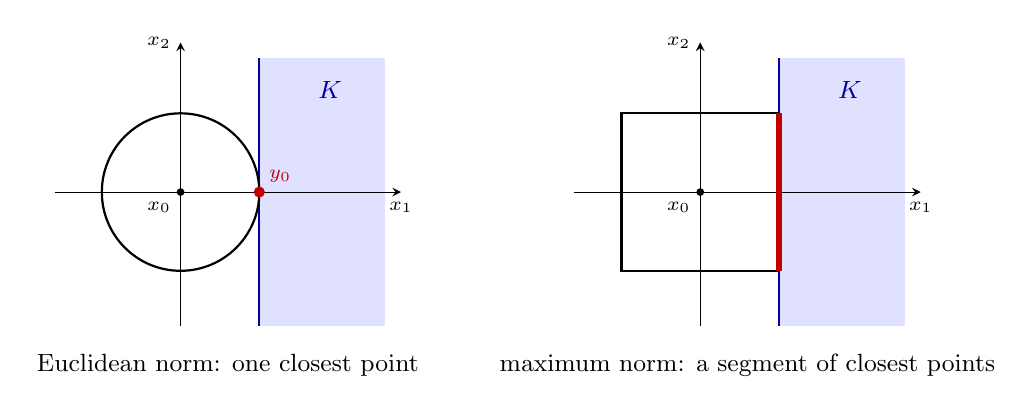
\begin{tikzpicture}[>=stealth]
  \begin{scope}
    \fill[blue!12] (1,-1.7) rectangle (2.6,1.7);
    \draw[blue!60!black, thick] (1,-1.7) -- (1,1.7);
    \draw[->] (-1.6,0) -- (2.8,0) node[below, font=\scriptsize] {$x_1$};
    \draw[->] (0,-1.7) -- (0,1.9) node[left, font=\scriptsize] {$x_2$};
    \draw[thick] (0,0) circle (1);
    \fill (0,0) circle (1.4pt) node[below left, font=\scriptsize] {$x_0$};
    \fill[red!75!black] (1,0) circle (2pt) node[above right, font=\scriptsize] {$y_0$};
    \node[blue!60!black, font=\small] at (1.9,1.3) {$K$};
    \node[font=\small] at (0.6,-2.2) {Euclidean norm: one closest point};
  \end{scope}
  \begin{scope}[xshift=6.6cm]
    \fill[blue!12] (1,-1.7) rectangle (2.6,1.7);
    \draw[blue!60!black, thick] (1,-1.7) -- (1,1.7);
    \draw[->] (-1.6,0) -- (2.8,0) node[below, font=\scriptsize] {$x_1$};
    \draw[->] (0,-1.7) -- (0,1.9) node[left, font=\scriptsize] {$x_2$};
    \draw[thick] (-1,-1) rectangle (1,1);
    \fill (0,0) circle (1.4pt) node[below left, font=\scriptsize] {$x_0$};
    \draw[red!75!black, line width=2pt] (1,-1) -- (1,1);
    \node[blue!60!black, font=\small] at (1.9,1.3) {$K$};
    \node[font=\small] at (0.6,-2.2) {maximum norm: a segment of closest points};
  \end{scope}
\end{tikzpicture}
